After running all these steps, you should see the following window:

\begin{center}
    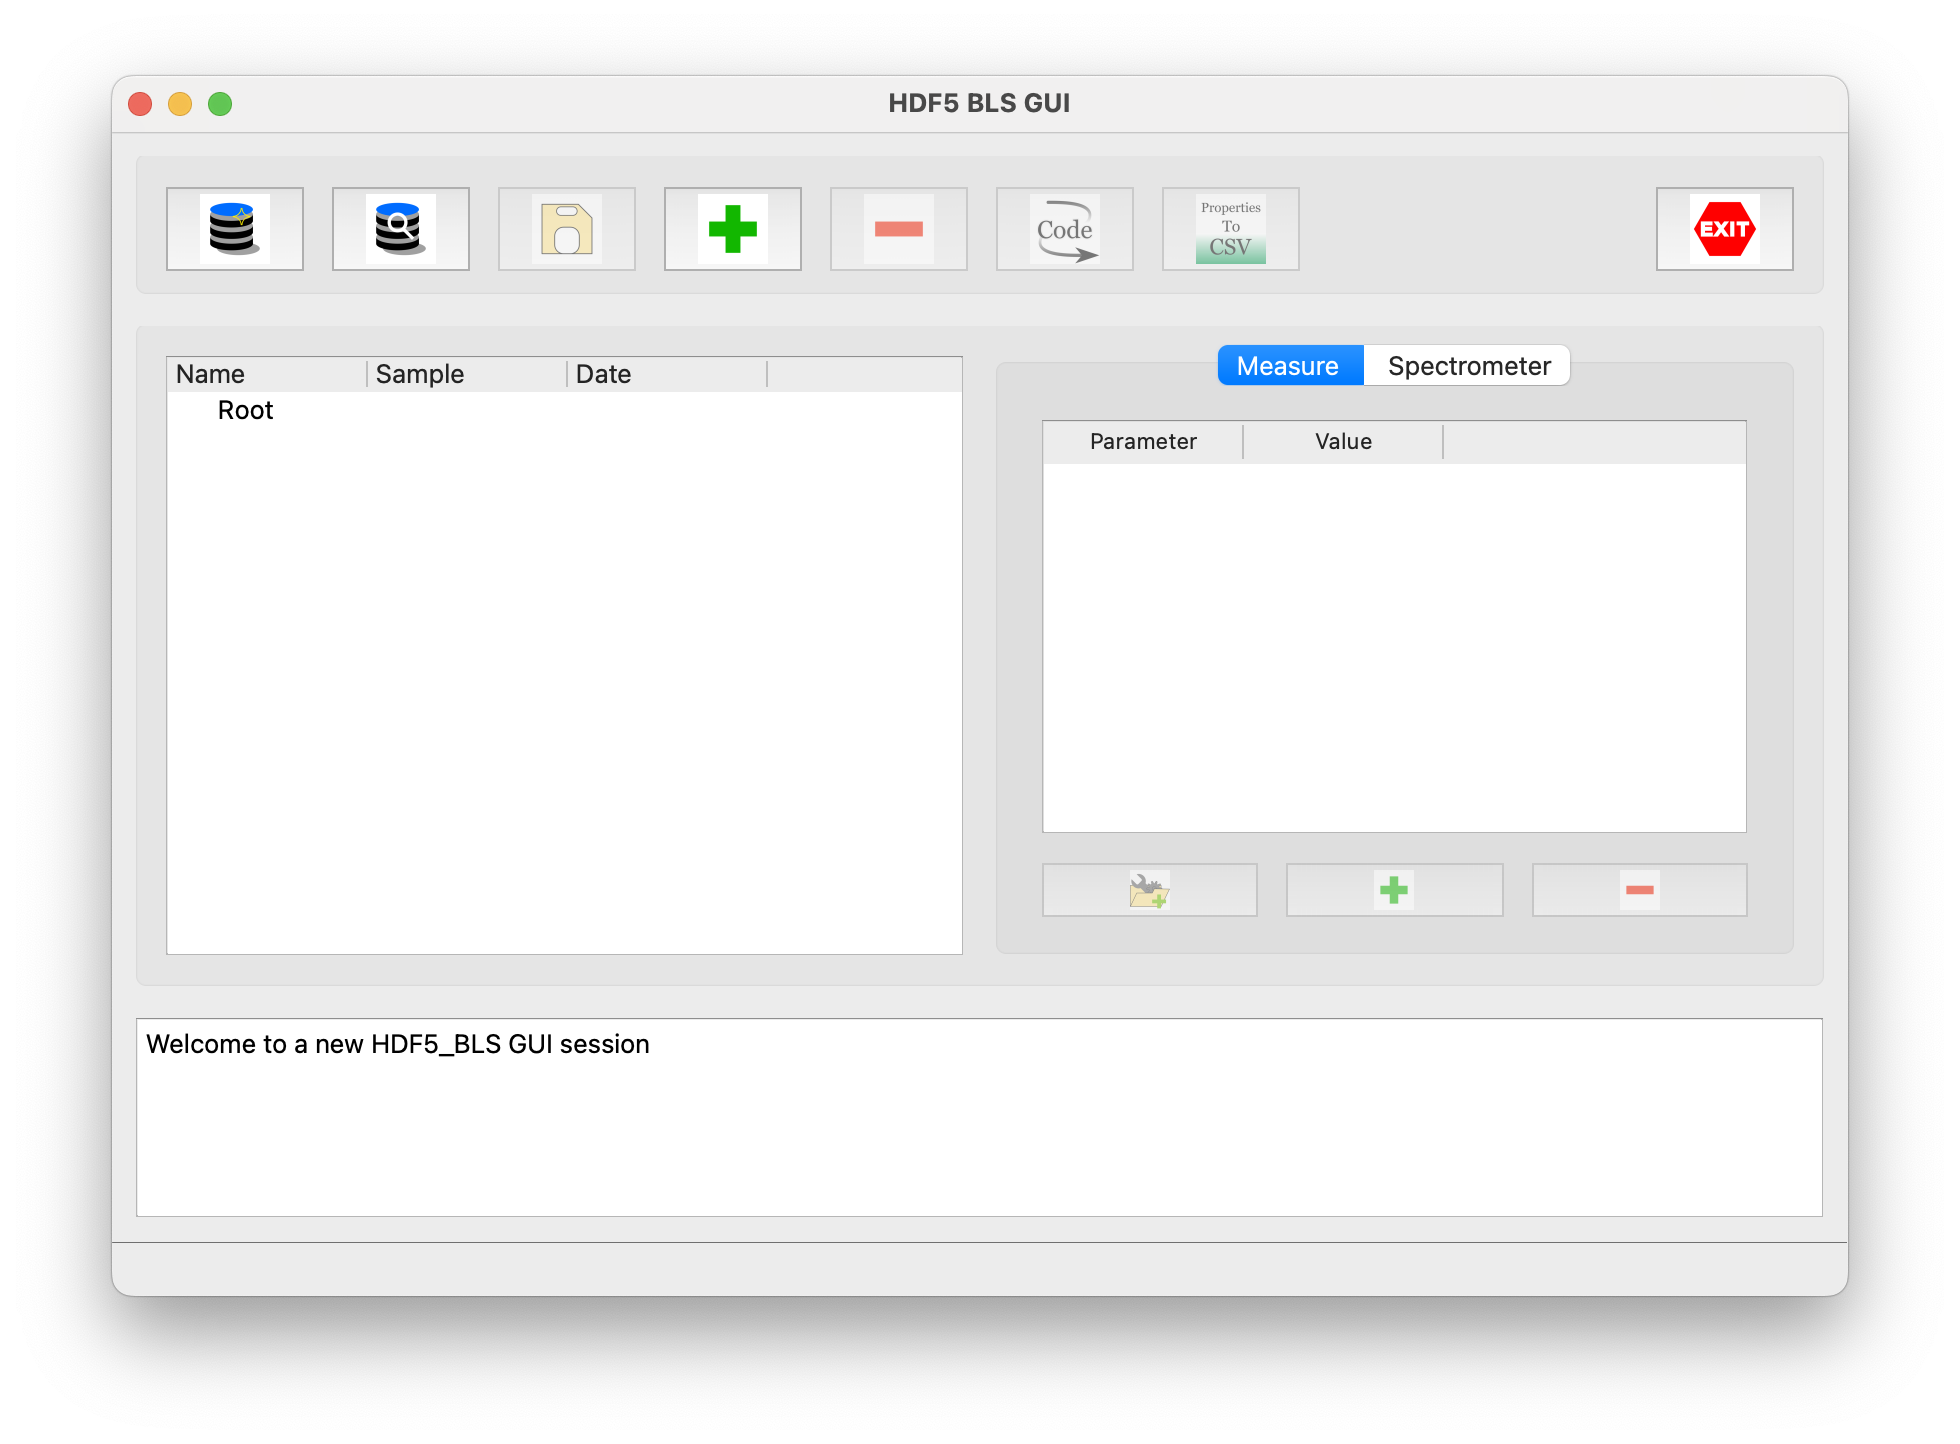
\includegraphics[width=\textwidth]{img/main_window.png}
\end{center}

You can then drag and drop your data into the left pannel and structure it as you wish. 

You can also add properties to your data in the form of a standard CSV file which model can be found in the \texttt{spreadsheets} folder of the repository. To add a new property file to your measure, select your measure on the left pannel and drag and drop your property file to the right pannel from a file viewer. 

Note that you can add property to a group of data. In that case, the property apply to all its elements.